\documentclass{standalone}

\usepackage{tikz}
\usetikzlibrary{positioning}
\usetikzlibrary{arrows,automata}
\usetikzlibrary{shapes,arrows,fit}

\begin{document}
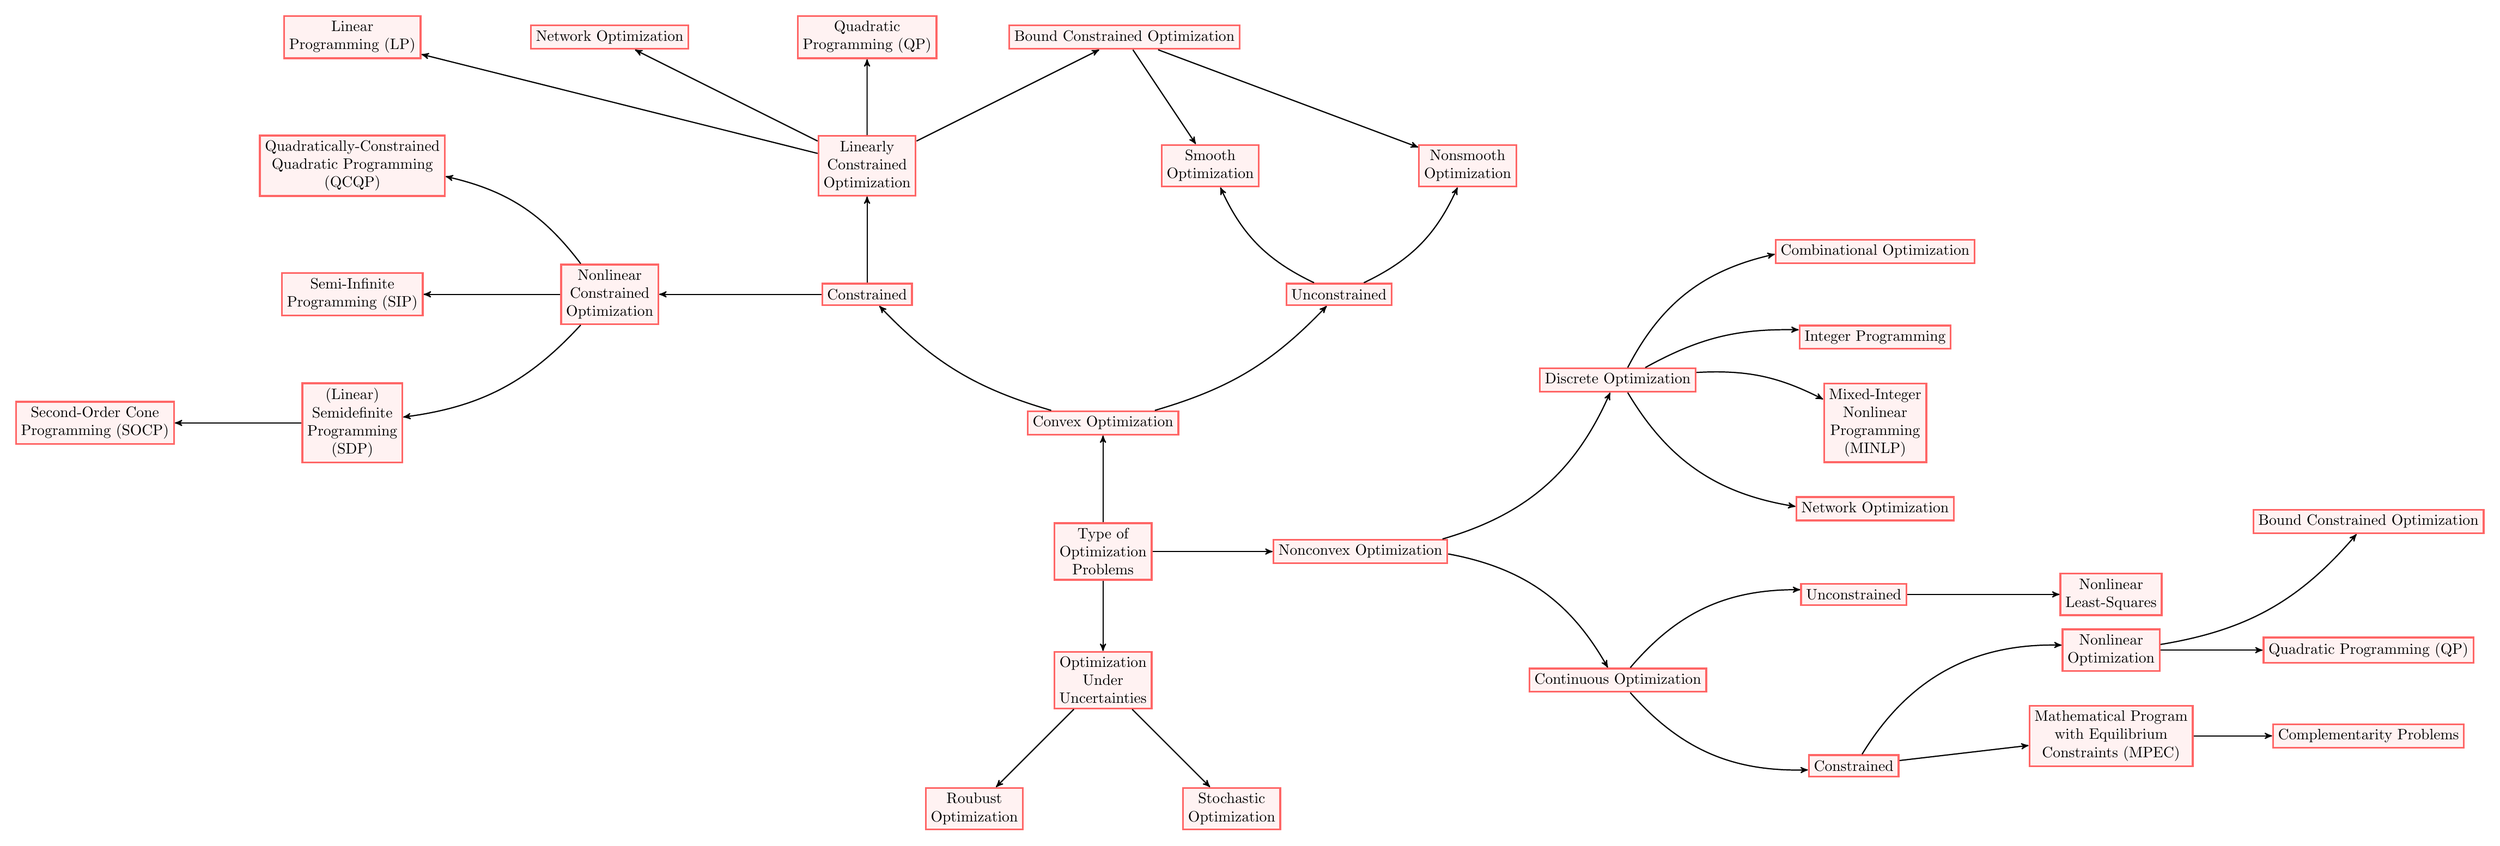
\begin{tikzpicture}[
    ->,
    >=stealth', % make the arrow's tip prettier
    auto,
    node distance=3cm,
    thick, % make the arrow's width thickier
    roundnode/.style={circle, draw=green!60, fill=green!5, very thick, minimum size=7mm},
    squarednode/.style={rectangle, draw=red!60, fill=red!5, very thick, minimum size=5mm},
    ]
    %Nodes
    \node[squarednode, align=center]      (opt)  {Type of\\Optimization\\Problems};
    
    % convex branch
    \node[squarednode]      (convex)          [above of=opt]                        {Convex Optimization};
    \node[squarednode]      (constrained)     [above of=convex, left of=convex, xshift=-2.5cm]    {Constrained};
    \node[squarednode]      (unconstrained)   [above of=convex, right of=convex, xshift=2.5cm]    {Unconstrained};
    %% constrained branch
    \node[squarednode, align=center]      (linconstopt)   [above of=constrained]    {Linearly\\Constrained\\Optimization};
    \node[squarednode, align=center]      (nonlinconstopt)   [left of=constrained, , xshift=-3cm]    {Nonlinear\\Constrained\\Optimization};

    %%% Linearly constrained optimization branch
    \node[squarednode, align=center]      (lp)   [left of=linconstopt, above of=linconstopt, xshift=-9cm]    {Linear\\Programming (LP)};
    \node[squarednode, align=center]  (network2) [right of=lp, xshift=3cm] {Network Optimization};
    \node[squarednode, align=center]  (qp) [right of=network2, xshift=3cm] {Quadratic\\Programming (QP)};
    \node[squarednode, align=center]  (boundconstopt) [right of=qp, xshift=3cm] {Bound Constrained Optimization};
    
    %% constrained branch
    \node[squarednode, align=center]      (smoothopt)   [above of=unconstrained, left of=unconstrained]    {Smooth\\Optimization};
    \node[squarednode, align=center]      (nsmoothopt)   [right of=smoothopt, xshift=3cm]    {Nonsmooth\\Optimization};
    
    %%% Nonlinear Constrained Optimization branch
    \node[squarednode, align=center]      (qcqp)   [left of=nonlinconstopt, above of=nonlinconstopt, xshift=-3cm]    {Quadratically-Constrained\\Quadratic Programming\\(QCQP)};
    \node[squarednode, align=center]      (sip)   [below of=qcqp]    {Semi-Infinite\\Programming (SIP)};
    \node[squarednode, align=center]      (sdp)   [below of=sip]    {(Linear)\\Semidefinite\\Programming\\(SDP)};
    %%%% Semidefinite Programming (SDP) branch
    \node[squarednode, align=center]      (socp)   [left of=sdp, xshift=-3cm]    {Second-Order Cone\\Programming (SOCP)};


    % nonconvex branch
    \node[squarednode]                  (nconvex)       [right of=opt, xshift=3cm]     {Nonconvex Optimization};
    \node[squarednode]                  (continuous)       [right of=nconvex, xshift=3cm, yshift=-3cm]     {Continuous 
    Optimization};
    \node[squarednode] (discrete) [right of=nconvex, xshift=3cm, yshift=4cm] {Discrete Optimization};
    %% discrete branch
    \node[squarednode]  (combinational) [right of=discrete, xshift=3cm, yshift=3cm] {Combinational Optimization};
    \node[squarednode]  (integer) [right of=discrete, xshift=3cm, yshift=1cm] {Integer Programming};
    \node[squarednode, align=center]  (minlp) [right of=discrete, xshift=3cm, yshift=-1cm] {Mixed-Integer\\Nonlinear\\Programming\\(MINLP)};
    \node[squarednode, align=center]  (network) [right of=discrete, xshift=3cm, yshift=-3cm] {Network Optimization};
    %% continuous branch
    \node[squarednode]      (cunconstrained)     [above of=continuous, right of=continuous, xshift=2.5cm, yshift=-1cm]    {Unconstrained};
    \node[squarednode]      (cconstrained)   [below of=continuous, right of=continuous, xshift=2.5cm, yshift=1cm]    {Constrained};
    %%% continuous branch unconstrained
    \node[squarednode, align=center]      (nls)     [right of=cunconstrained, xshift=3cm]    {Nonlinear\\Least-Squares};
    %%% continuous branch constrained
    \node[squarednode, align=center]      (nopt)     [right of=cconstrained, above of=cconstrained, xshift=3cm, yshift=-0.3cm]    {Nonlinear\\Optimization};
    \node[squarednode, align=center]      (mpec)     [below of=nopt, yshift=1cm]    {Mathematical Program\\with Equilibrium\\Constraints (MPEC)};
    %%%% MPEC branch
    \node[squarednode, align=center]      (complementarity)     [right of=mpec, xshift=3cm]    {Complementarity Problems};
    %%%% nop branch
    \node[squarednode, align=center]      (qp2)     [right of=nopt, xshift=3cm]    {Quadratic Programming (QP)};
    \node[squarednode, align=center]      (boundconstopt2)     [right of=nopt, above of=nopt, xshift=3cm]    {Bound Constrained Optimization};


    % underuncert branch
    \node[squarednode, align=center]      (underuncert)   [below of=opt]                 {Optimization\\Under\\Uncertainties};
    \node[squarednode, align=center]      (roubust)   [below of=underuncert,left of=underuncert]                 {Roubust\\Optimization};
    \node[squarednode, align=center]      (stochastic)   [below of=underuncert,right of=underuncert]                 {Stochastic\\Optimization};

    
    \path[every node/.style={font=\sffamily\small}]
    % lines from opt
    (opt) edge node [right] {} (nconvex)
    (opt) edge node [below] {} (underuncert)
    (opt) edge node [above] {} (convex)
    % lines from convex
    (convex) edge[bend left=15] node [above] {} (constrained)
    (convex) edge[bend right=15] node [above] {} (unconstrained)
    % lines from unconstrained
    (unconstrained) edge[bend left=20] node [above] {} (smoothopt)
    (unconstrained) edge[bend right=20] node [above] {} (nsmoothopt)
    % lines from constrained
    (constrained) edge node [above] {} (linconstopt)
    (constrained) edge node [left] {} (nonlinconstopt)
    % lines from linconstopt
    (linconstopt) edge node [above] {} (lp)
    (linconstopt) edge node [above] {} (network2)
    (linconstopt) edge node [above] {} (boundconstopt)
    (linconstopt) edge node [above] {} (qp)
    % lines from boundconstopt
    (boundconstopt) edge node [] {} (smoothopt)
    (boundconstopt) edge node [] {} (nsmoothopt)
    % lines from nonlinconstopt
    (nonlinconstopt) edge[bend right=20] node [left] {} (qcqp)
    (nonlinconstopt) edge[] node [left] {} (sip)
    (nonlinconstopt) edge[bend left=20] node [left] {} (sdp)
    % lines from sdp
    (sdp) edge[] node [] {} (socp)
    % lines from underuncert
    (underuncert) edge node [] {} (roubust)
    (underuncert) edge node [] {} (stochastic)
    % lines from nconvex
    (nconvex) edge[bend left=25] node [right] {} (continuous)
    (nconvex) edge[bend right=25] node [right] {} (discrete)
    % lines from discrete
    (discrete) edge[bend left=25] node [right] {} (combinational)
    (discrete) edge[right, bend left=15] node [left] {} (integer)
    (discrete) edge[right, bend left=15] node [left] {} (minlp)
    (discrete) edge[right, bend right=25] node [left] {} (network)
    % lines from continuous
    (continuous) edge[bend left=25] node [right] {} (cunconstrained)
    (continuous) edge[bend right=25] node [right] {} (cconstrained)
    % lines from cunconstrained
    (cunconstrained) edge[] node [right] {} (nls)
    % lines from cconstrained
    (cconstrained) edge[bend left] node [right] {} (nopt)
    (cconstrained) edge[] node [right] {} (mpec)
    % lines from mpec
    (mpec) edge[] node [right] {} (complementarity)
    % lines from nopt
    (nopt) edge[] node [right] {} (qp2)
    (nopt) edge[bend right=20] node [right] {} (boundconstopt2);
\end{tikzpicture}
\end{document}